La figura \ref{fig:mc_h1} muestra la probabilidad de error para ambos sistemas en base a una simulación Montecarlo, y las curvas teóricas para comparar. Se tomo un valor de $h=1$.

\begin{figure}[]
    \centering
    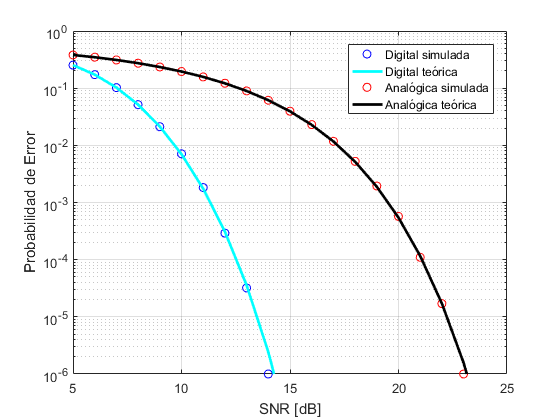
\includegraphics[width=\textwidth]{./Matlab/ej4h=1n=1meg.png}
    \caption{Probabilidad de error en función del SNR, simulada y teórica. }
\label{fig:prob_err}
\end{figure}

Puede verse que las curvas teóricas corresponden con muy buena precisión a los puntos simulados. Esto se debe a que, al generarse una cantidad muy grande de entradas simuladas, el cociente de errores y realizaciones aproxima estadísticamente la probabilidad del error.

En particular, este gráfico se generó con un millón de realizaciones para cada sistema y valor de \textbf{SNR}; sin embargo, se observó que a partir de aproximadamente veinte mil realizaciones puede notarse una clara tendencia a aproximarse a las curvas teóricas. 